\section{Testen}
\label{Beispiel-Nutzung}

%% describes an exampe of Usage
%% schaltkreis, messwerte, etc.
%% von Schwingkreis (LC-Circuit)
Im Folgenden wird das Oszilloskop und seine Funktionen getestet.
Dafür wird zuerst eine Beispielmessung von einem Kondensator im Gleichstromkreis durchgeführt. \newline
Danach wird eine sinusartige Spannung gemessen und geschaut, ob das Oszilloskop den Anforderungen genügt.
Dafür wird es zusätzlich mit einem kommerziellen Oszilloskopen, im Hinblick auf die Messung, verglichen.

\subsection{Beispiel: Kondensator Ladevorgang}
\label{Kondensator Ladevorgang}
Der schematische Aufbau des Gleichstromkreises sieht wie folgt aus:
\begin{figure}[h]
	\centering
	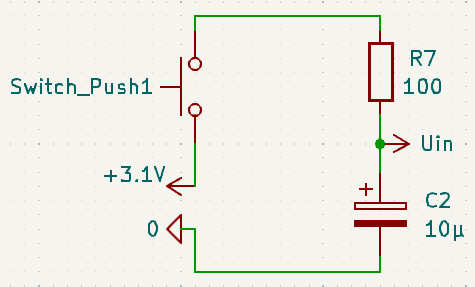
\includegraphics[width=0.5\textwidth]{images/schematic_beispielnutzung_kondensator2.png}
	\caption{Ladevorgangs eines Kondensators}
\end{figure}
\newline
Für die Messung, muss das Oszilloskop zur gemessenen Spannung parallel geschalten werden,
damit die Spannung am Oszilloskop die gleiche ist, wie die am gemessenen Stromkreis.
$U_{in}$ bezeichnet hierbei den Messeingang des Oszilloskops aus \ref{Gesamte_Schematic}
und $0$ ist der gemeinsame Ground aus dem Gleichstromkreis.
Um die Messung zu starten müssen der \textit{Btn3} auf dem Extension Board und \textit{Switch\_Push}
im Gleichstromkreis möglichst zeitgleich betätigt werden.
Die gemessene Spannungskurve ist in \autoref{Kondesator Messung selbstgebaut} zu sehen.
\begin{figure}[h!]
	\centering
	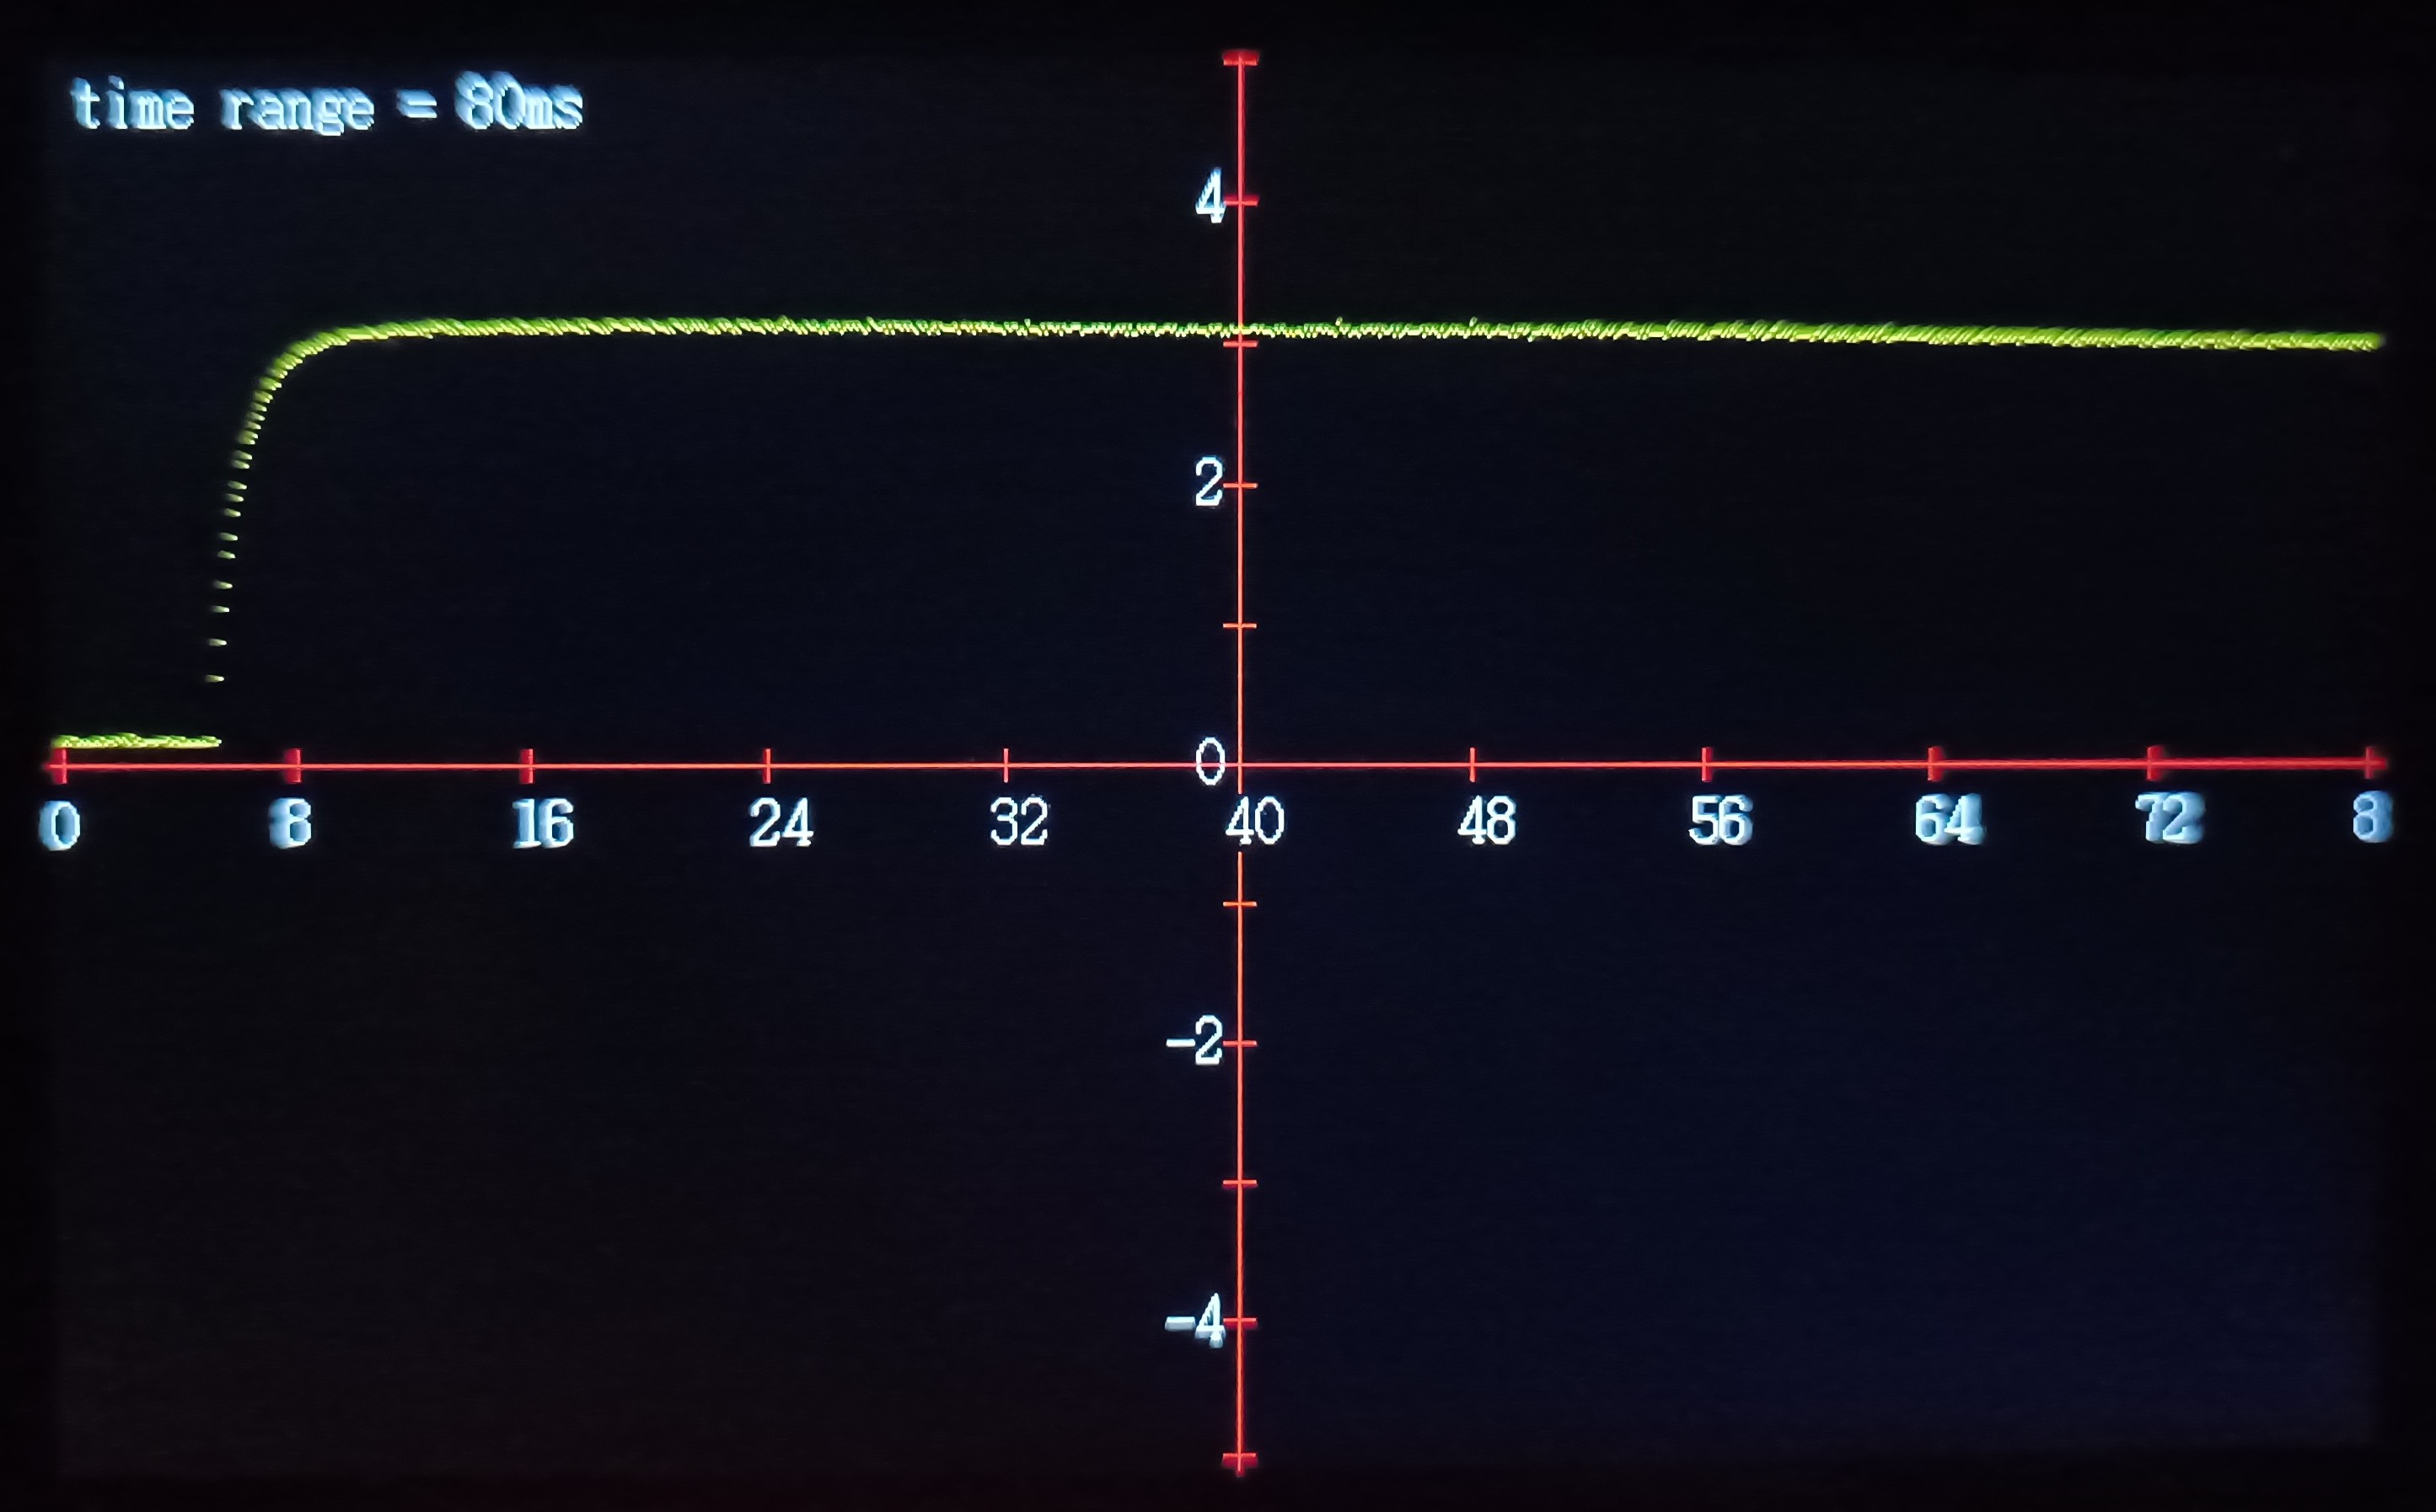
\includegraphics[width=0.5\textwidth]{images/messung_kondensator_ladekurve_selbstgebaut2.jpg}
	\caption{Messung des Ladevorgangs eines $10\mu F$ Kondensators im Gleichstromkreis}
	\label{Kondesator Messung selbstgebaut}
\end{figure}
\newline
Für die Spannung am Kondensator gilt, laut \cite{Kondensator_Ladekurve}:
$$
U_{in}(t) = U_0 \cdot (1 - e^{- \frac{t}{RC}})
$$
mit $U_0 = 3.1V$, $R=100 \Omega$, $C = 10\mu F$.
Daher ergibt sich theoretisch für $t=0.1s$, also am rechten Rand des Displays, $U_{in}(0.1s) = 3.1V$
und praktisch werden diese ungefähr auch gemessen.
%\newpage \noindent
%Zum Vergleich wird hier ein \textit{Tenma 72-8727} Oszilloskop, für die gleiche Messung, benutzt:
%\begin{figure}[h]
%	\centering
%	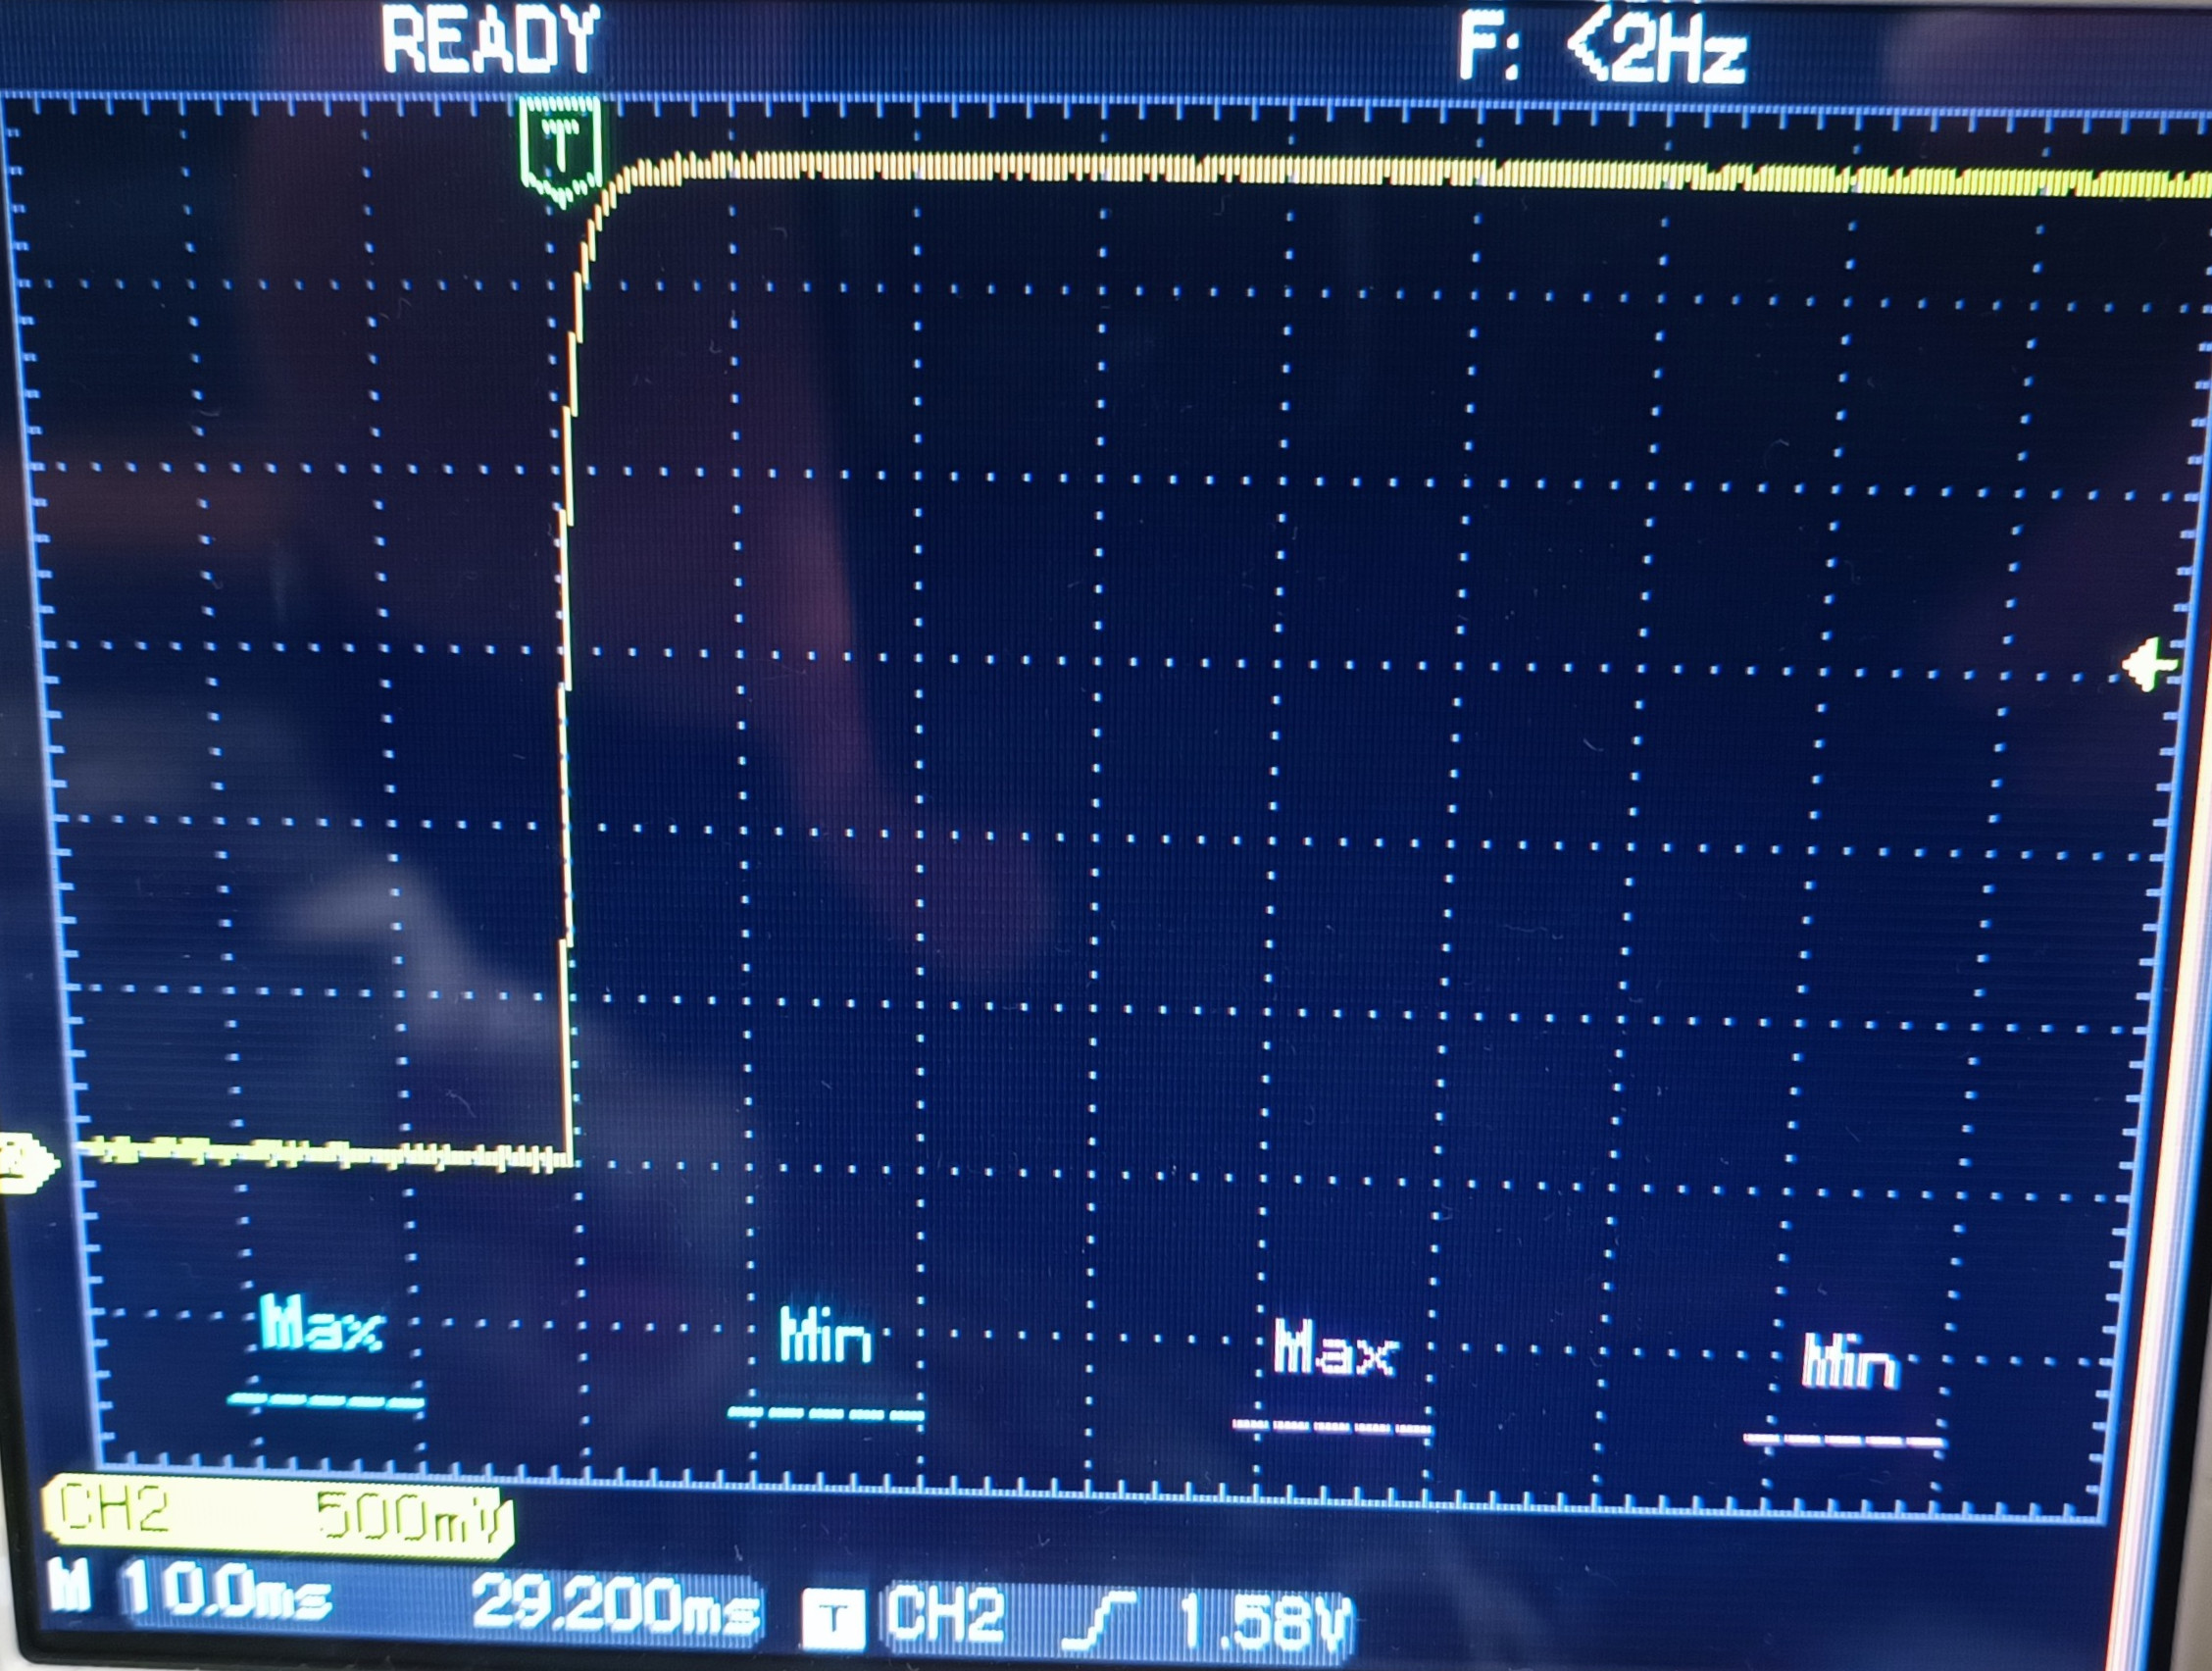
\includegraphics[width=0.7\textwidth]{images/messung_kondensator_ladekurve_profi3.jpg}
%	\caption{Gleiche Messung wie oben, aber mit einem kommerziellen Oszilloskop}
%\end{figure}


\subsection{Validierung der Anforderungen}
Nun soll geprüft werden, ob das Oszilloskop die Anforderungen aus \ref{Anforderungen} erfüllt.
Hierfür wird eine sinusartige Spannung aus einem Funktionsgenerator mit dem selbstgebauten
und dem kommerziellen \textit{Tenma 72-8727} Oszilloskopen gemessen
und deren Spannungskurven verglichen.


\subsubsection{Versuchsaufbau}
In diesem Versuch wird die Versorgungsspannung von $V^-_{CC} = -15V$ und $V^+_{CC} = +15V$
für die OpAmps aus einem Labornetzteil entnommen. Der Stepup Spannungswandler aus \ref{Gesamte_Schematic},
der dies übernehmen sollte, fällt hier weg. \newline
Für den Versuch wird an den Messeingängen der Oszilloskope ein Funktionsgenerator angeschlossen.
Dieser generiert eine Wechselspannung mit einer Amplitude von etwa $5V$ und Frequenz von $210\si{\hertz}$.
Diese Spannungskurve wird im folgenden gemessen.

%\subsubsection{Versuchsdurchführung}
%weiß nicht ob das hier noch reinkommt

\subsubsection{Messdaten}
Das Oszilloskop \textit{Tenma 72-8727} misst dabei folgende Werte:
\begin{figure}[h]
	\centering
	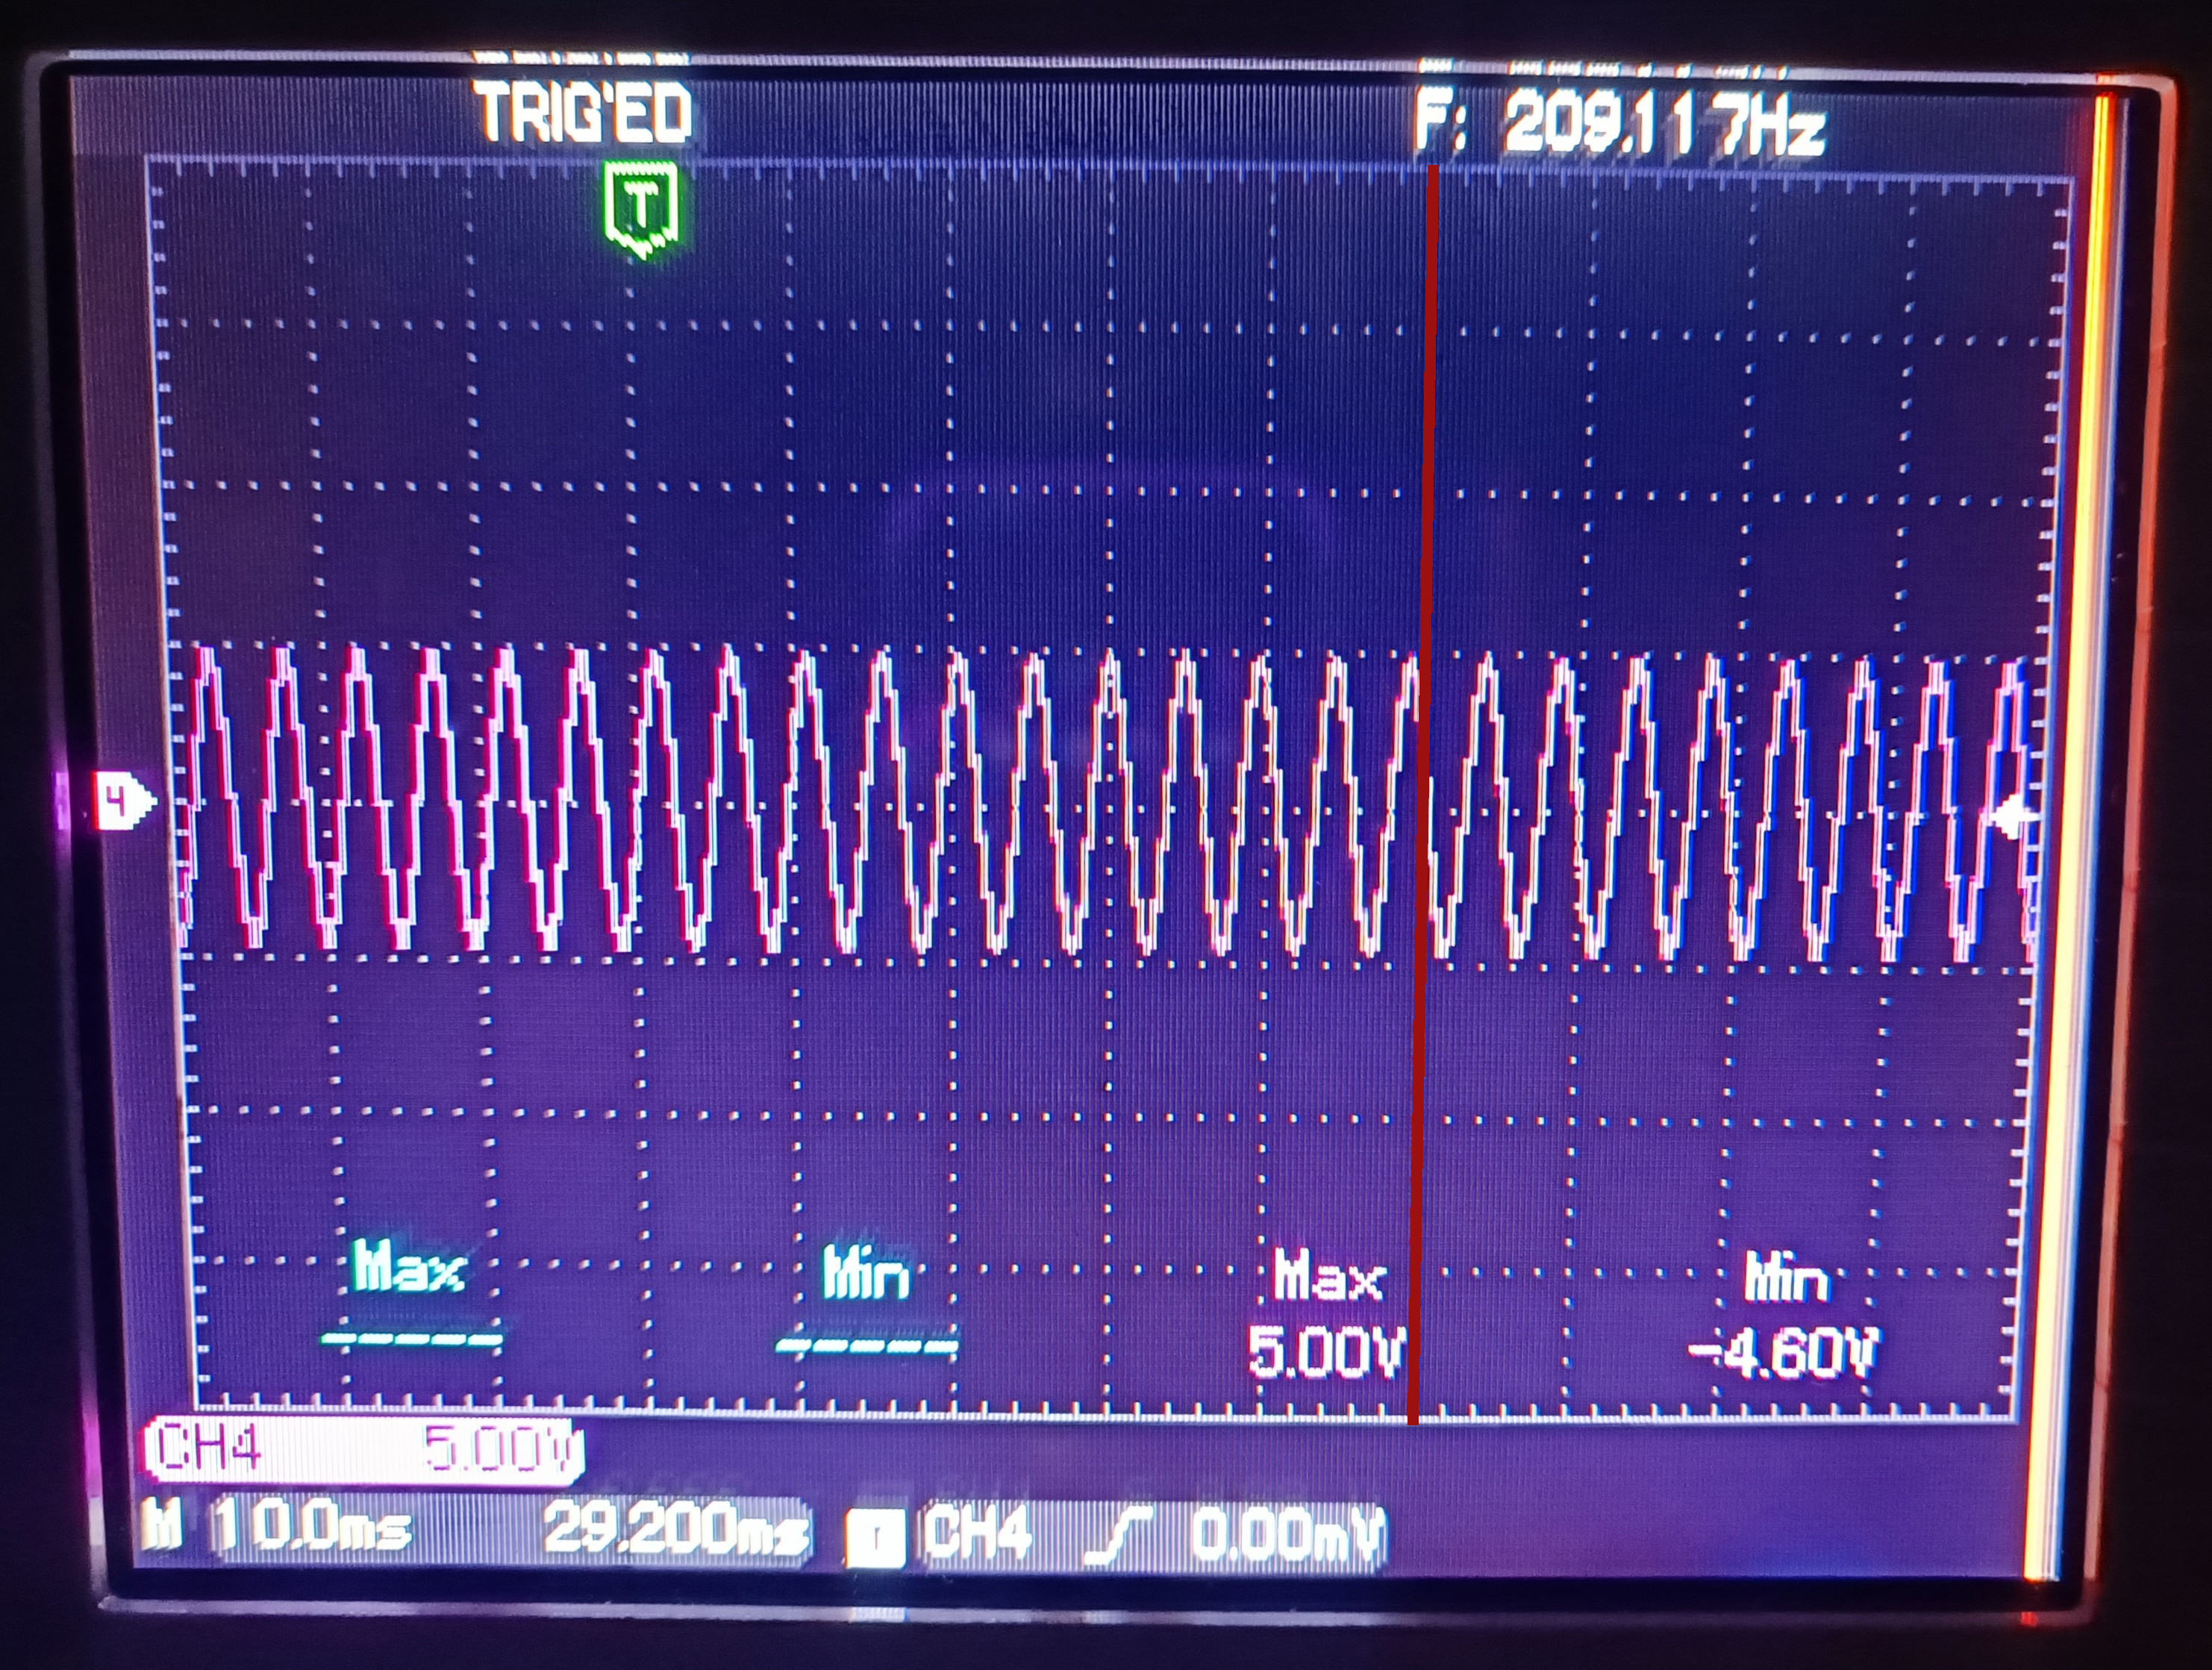
\includegraphics[width=0.6\textwidth]{images/sinus_profi_rot.jpg}
	\caption{Messung der Wechselspannung durch das \textit{Tenma 72-8727}}
	\label{Tenma Messung}
\end{figure}
\newline
Das Display hat in diesem Versuch einen Darstellungsbereich von $120\si{\milli s}$.
Die rote senkrechte Linie gibt die Zeit $t=80\si{\milli s}$ an, um den Darstellungsbereich mit dem
des selbstgebauten Oszilloskops zu vergleichen.
In diesem Zeitbereich werden in \autoref{Tenma Messung} $16$ Perioden gezählt.
Desweiteren  liegt die Amplitude bei ungefähr $5V$. \newline
Das selbstgebaute Oszilloskop misst folgendes:
\begin{figure}[h]
	\centering
	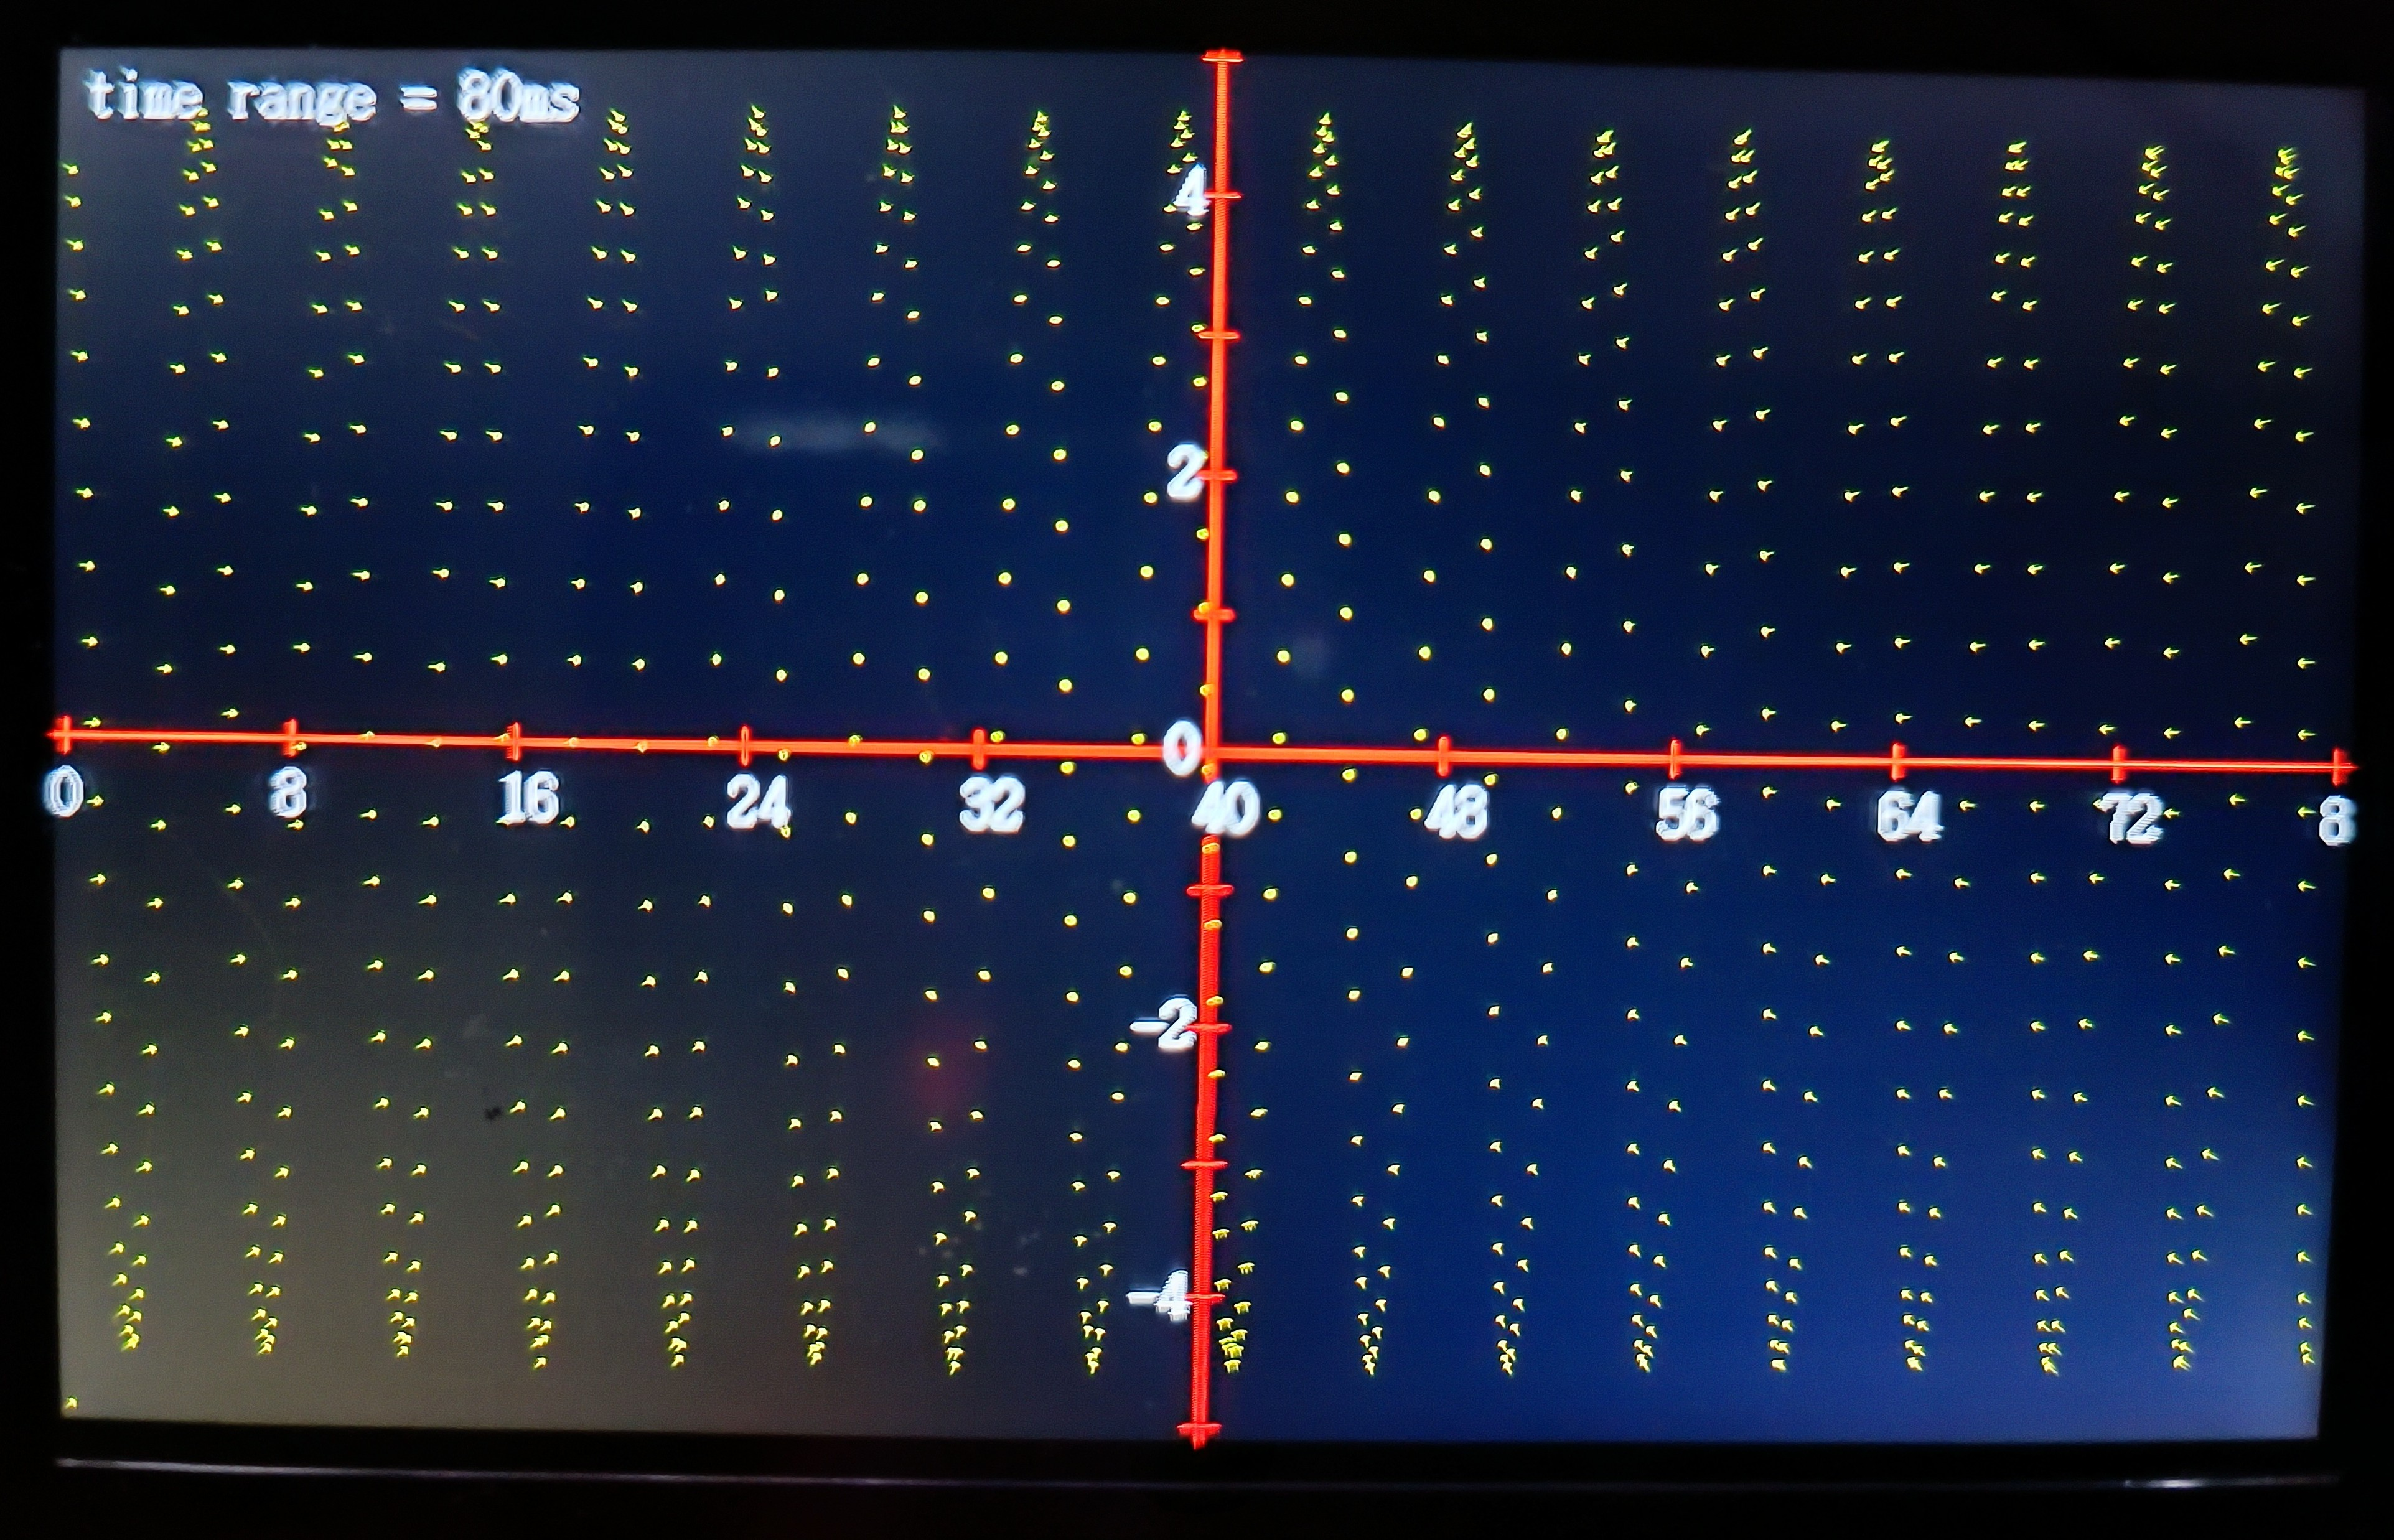
\includegraphics[width=0.7\textwidth]{images/sinus_selbstgebaut.jpg}
	\caption{Messung der Wechselspannung durch das selbstgebaute Oszilloskop}
	\label{Selbstgebaut Messung}
\end{figure}
\newline
Der zeitliche Darstellungsbereich beträgt $80\si{\milli s}$.
Dieser ist, im Gegensatz zum kommerziellen Oszilloskop, nicht variabel.
Das Display zeigt dabei ebenfalls $16$ Perioden und eine Amplitude von etwa $5V$.
\autoref{Selbstgebaut Messung} zeigt aber deutlich, dass das selbstgebaute Oszilloskop nur die einzelnen Punkte
darstellt und diese, anders als beim \textit{Tenma 72-8727}, nicht miteinander verbunden werden.
Die Messwerte als einzelne Punkte darzustellen ist bei großen Frequenzen unübersichtlich.
Aus verschiedenen Messungen ergab sich, dass das Oszilloskop, bis zu einer
Frequenz von ca. $700 \si{\hertz}$, übersichtliche Messwerte anzeigt.
Um die Display Ausgabe beider Oszilloskope besser vergleichen zu können, werden diese in einem Bildbearbeitungsprogramm (GIMP) gleich groß skaliert und übereinander gelegt:
\begin{figure}[h]
	\centering
	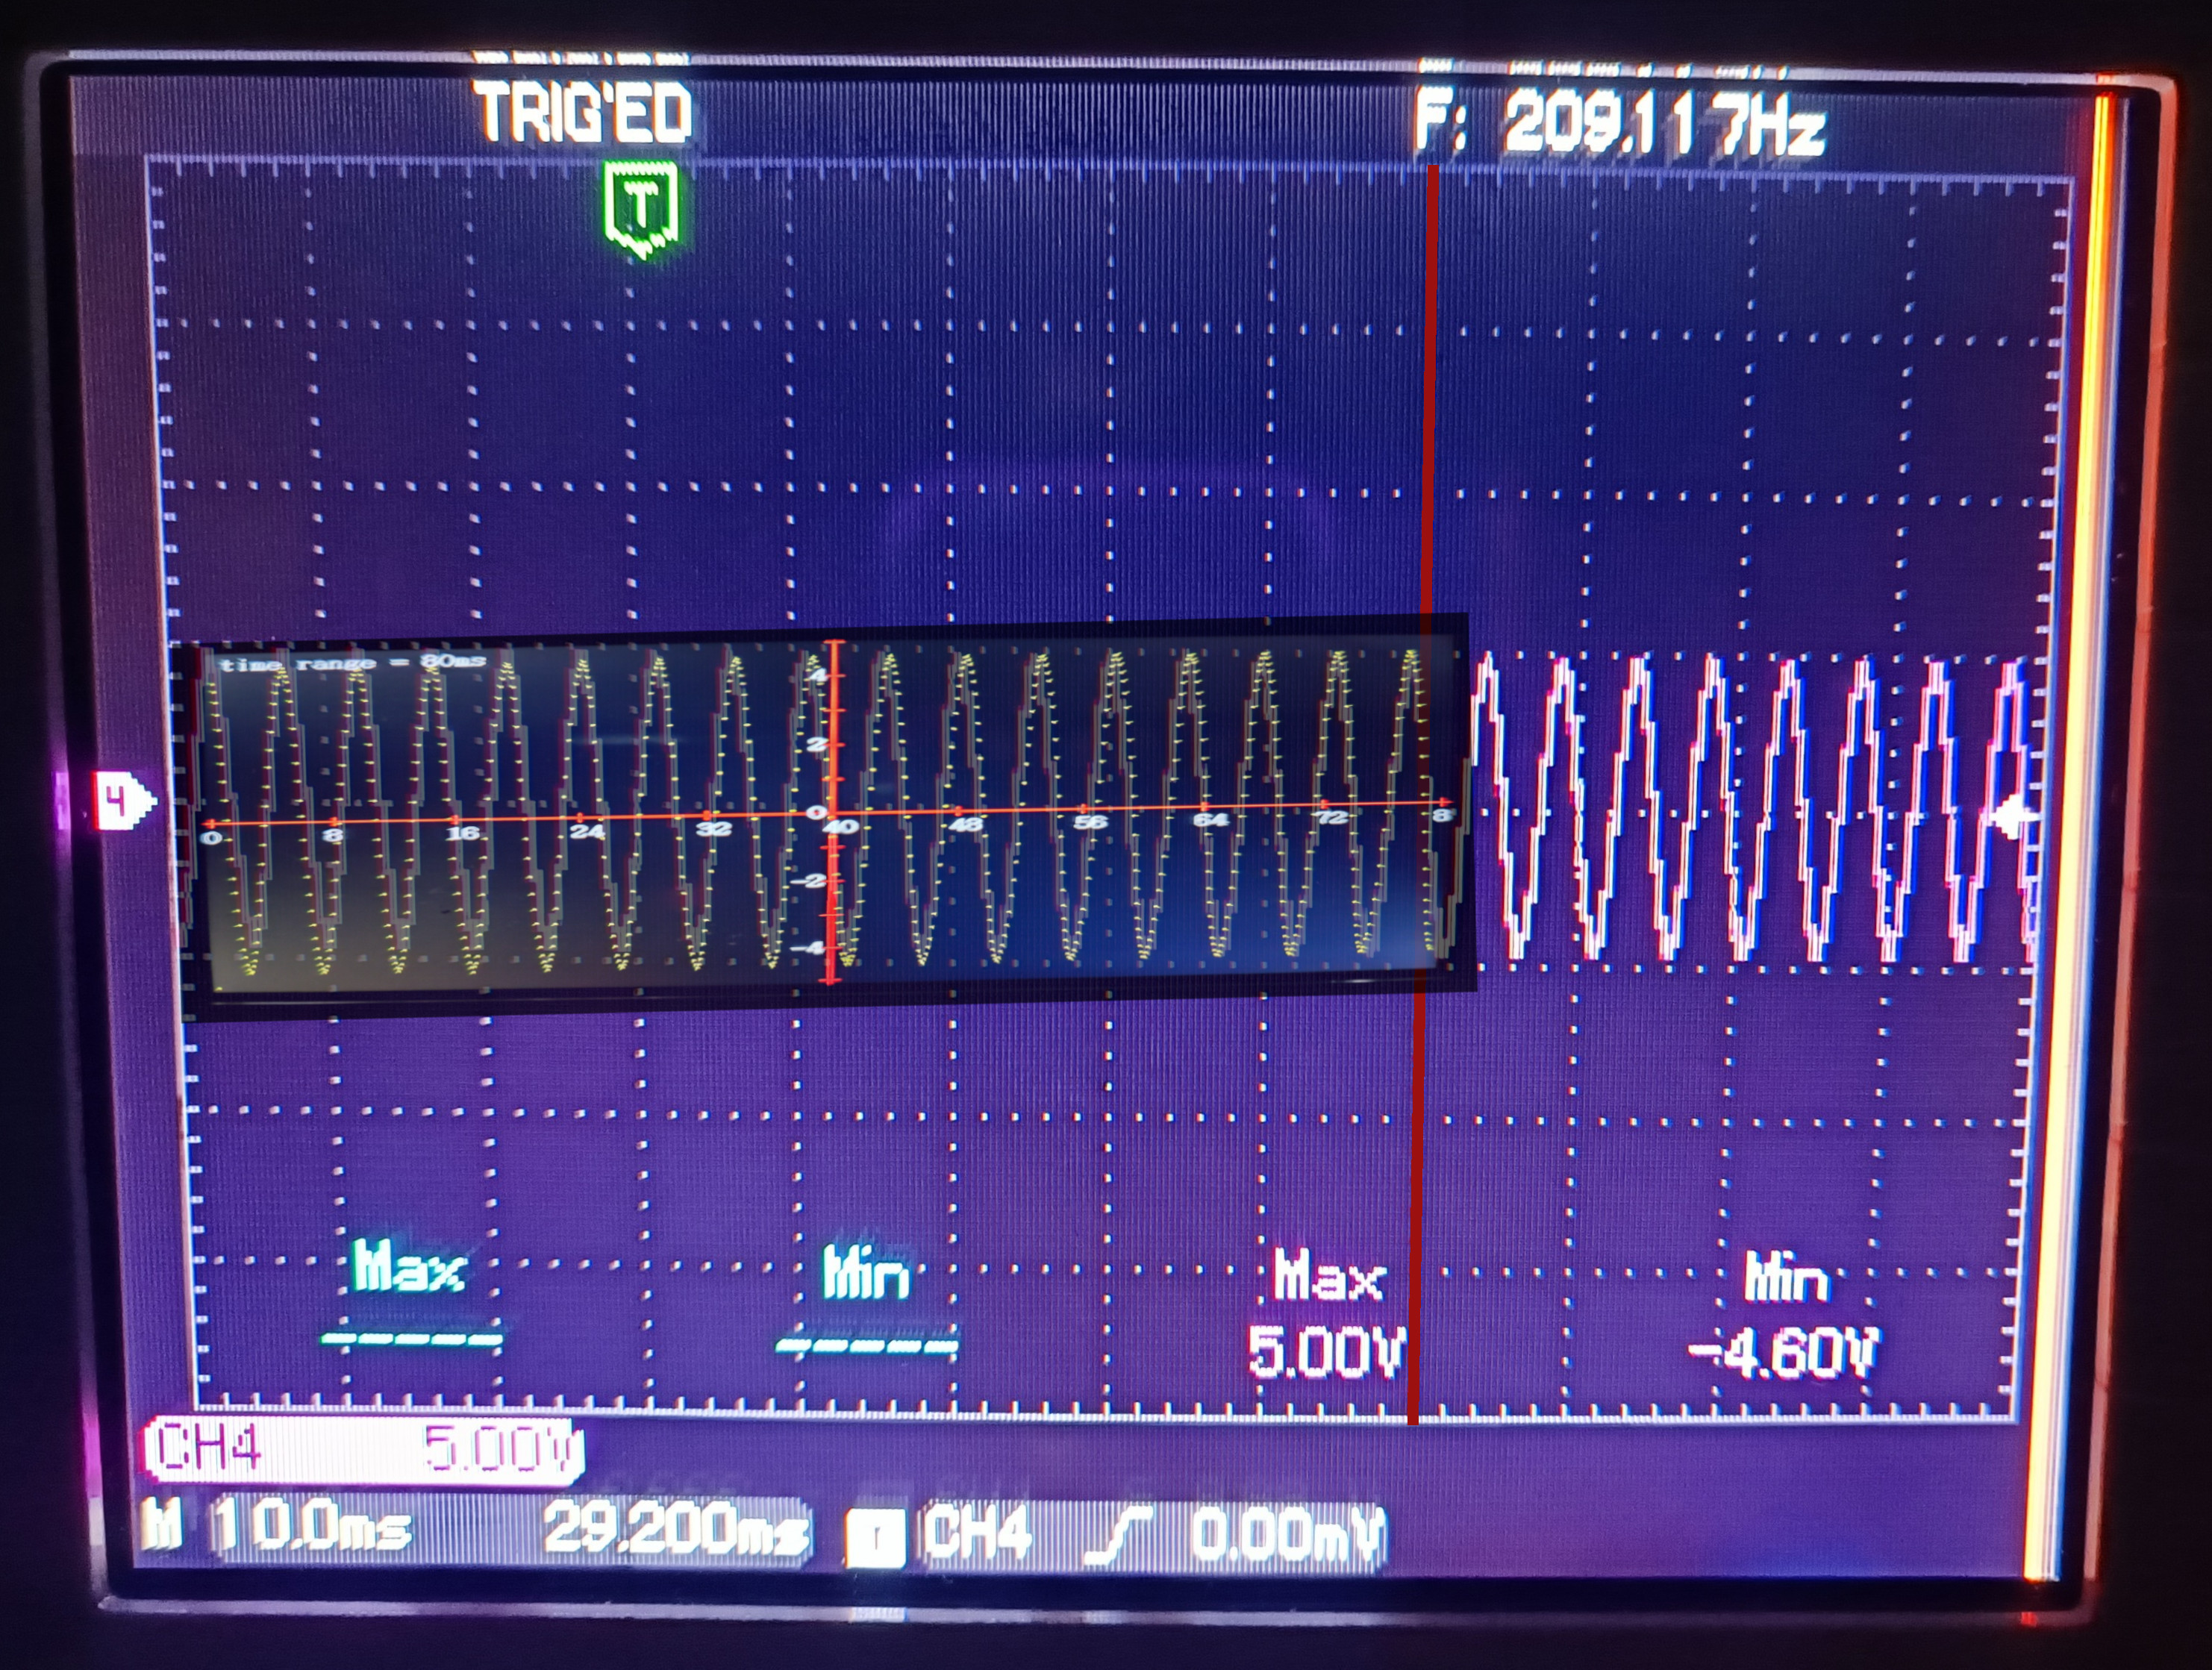
\includegraphics[width=0.7\textwidth]{images/sinus_uebereinander.jpg}
	\caption{\autoref{Tenma Messung} und \autoref{Selbstgebaut Messung} in GIMP bildlich übereinander gelegt}
\end{figure}
\newline
Die Abbildungen müssen hierfür skaliert und verschoben werden, weil die Oszilloskope nicht den selben Darstellungsbereich auf dem Display haben und nicht zur selben Zeit getriggert wurden.
Zudem wurden die Displays nicht im selben Winkel abfotografiert.
Durch die Bildbearbeitung stimmen die Spannungskurven bildlich überein.
Das Ergebnis des selbstgebauten Oszilloskops sieht sehr nach dem des \textit{Tenma 72-8727}, bezüglich der Steigung, Amplitude und Frequenz der Spannungskurven, aus.


\subsubsection{Auswertung}
Das selbstgebaute Oszilloskop misst im Versuch ähnlich dem \textit{Tenma 72-8727}.
Die Anforderung an den Spannungsbereich der Messung von $[-5, 5] V$ wurden somit erfüllt.
Ebenfalls wurde eine Messfrequenz von $10 \si{\kilo \hertz}$ erreicht.
Das Display zeigt einen zeitliche Darstellungsbereich von $80\si{\milli s}$ an.
Dementsprechend erfüllt das Oszilloskop die, in Abschnitt \ref{Anforderungen} gestellten, Anforderungen.

